\documentclass[border=4pt,12pt]{standalone}
% House style for redrawn exam diagrams (diagram-v4: 0.4pt lines, filled -latex arrows, fine dashes; stipple and hatching drawn as real dots/lines (no PDF/SVG patterns, so they render in every browser and at any scale); transparent background). Every figure \input's this.
\usepackage{amsmath,amssymb}
\usepackage{txfonts}
\usepackage{pdfrender,xcolor}
% \halo{text}: label on shading. The shading stops just around each letter's outline (a thin knock-out that follows the
% glyphs, like the papers' typesetting), never a box. Owner: "I don't want a box around the text".
\newcommand{\halo}[1]{\leavevmode\rlap{\pdfrender{TextRenderingMode=2,LineWidth=2.2pt,LineJoinStyle=1,StrokeColor=white,FillColor=white}#1}#1}
\usepackage{tikz,pgfplots}
\pgfplotsset{compat=1.18}
\usetikzlibrary{arrows.meta,calc,angles,quotes,patterns,patterns.meta,intersections,positioning,decorations.markings,shapes.geometric}
% Stipple and hatching are drawn as actual dots / lines clipped to the region (path picture), NOT as pattern fills:
% SVG <pattern> fills vanish or blur when browsers scale the image, so the owner could not see the shading.
% Each dot is a 0.72pt square (keeps SVGs small; reads as a dot at print size). Dots sit on one global staggered grid, so neighbouring regions line up.
\makeatletter
\newdimen\ex@x \newdimen\ex@y \newdimen\ex@xa \newdimen\ex@ya \newdimen\ex@xb \newdimen\ex@yb \newcount\ex@row
\def\exam@stipplecolor{black!75}\def\exam@dotr{0.42pt}\def\exam@dotgap{2.5}
\def\ex@rowdots{\ifdim\ex@x<\ex@xb \pgfpathrectangle{\pgfqpoint{\dimexpr\ex@x-0.36pt\relax}{\dimexpr\ex@y-0.36pt\relax}}{\pgfqpoint{0.72pt}{0.72pt}}\advance\ex@x by \exam@dotgap pt\relax\expandafter\ex@rowdots\fi}
\def\exam@stipple{%
  \pgftransformreset% dots are sized in real points even inside scaled pictures
  \pgfpointanchor{path picture bounding box}{south west}\ex@xa=\pgf@x \ex@ya=\pgf@y
  \pgfpointanchor{path picture bounding box}{north east}\ex@xb=\pgf@x \ex@yb=\pgf@y
  \pgfsetfillcolor{\exam@stipplecolor}\pgfmathsetmacro\ex@h{\exam@dotgap/2}%
  \pgfmathtruncatemacro\ex@r{floor(\ex@ya/\ex@h)-1}\ex@row=\ex@r\relax
  \ex@y=\ex@r\dimexpr\ex@h pt\relax
  \loop\ifdim\ex@y<\ex@yb
    \pgfmathtruncatemacro\ex@c{floor(\ex@xa/\exam@dotgap)-1}\ex@x=\ex@c\dimexpr\exam@dotgap pt\relax
    \ifodd\ex@row \advance\ex@x by \ex@h pt\fi
    \ex@rowdots
    \advance\ex@y by \ex@h pt \advance\ex@row by 1
    \ifnum\numexpr\ex@row-(\ex@row/4)*4\relax=0 \pgfusepath{fill}\fi% flush every 4 rows: bounded TeX memory, few clip copies in the SVG
  \repeat\pgfusepath{fill}}
\newdimen\ex@d
\def\exam@hatch#1{% #1 = 1 for /, -1 for \ ; lines 45 degrees, 3pt apart
  \pgftransformreset
  \pgfpointanchor{path picture bounding box}{south west}\ex@xa=\pgf@x \ex@ya=\pgf@y
  \pgfpointanchor{path picture bounding box}{north east}\ex@xb=\pgf@x \ex@yb=\pgf@y
  \ex@d=\dimexpr\ex@yb-\ex@ya\relax \ex@x=\dimexpr\ex@xa-\ex@d\relax
  \loop\ifdim\ex@x<\ex@xb
    \ifnum#1>0 \pgfpathmoveto{\pgfqpoint{\ex@x}{\ex@ya}}\pgfpathlineto{\pgfqpoint{\dimexpr\ex@x+\ex@d\relax}{\ex@yb}}%
    \else \pgfpathmoveto{\pgfqpoint{\ex@x}{\ex@yb}}\pgfpathlineto{\pgfqpoint{\dimexpr\ex@x+\ex@d\relax}{\ex@ya}}\fi
    \advance\ex@x by 4.24pt
  \repeat
  \pgfsetlinewidth{0.4pt}\pgfsetstrokecolor{black}\pgfusepath{stroke}}
\def\examstipple{\exam@stipple}\def\examhatch{\exam@hatch}\def\examsetstipplecolor#1{\def\exam@stipplecolor{#1}}\def\examsetdotgap#1{\def\exam@dotgap{#1}}
\makeatother
% (legacy pattern kept for old files)
% staggered stipple like the NESA papers' dotted shading
\pgfdeclarepatternformonly{exam stipple}{\pgfpointorigin}{\pgfqpoint{2.2pt}{2.2pt}}{\pgfqpoint{2.2pt}{2.2pt}}{%
  \pgfpathcircle{\pgfqpoint{0.55pt}{0.55pt}}{0.42pt}\pgfpathcircle{\pgfqpoint{1.65pt}{1.65pt}}{0.42pt}\pgfusepath{fill}}
\tikzset{
  every picture/.style={line width=0.6pt, >={Latex[length=2mm,width=1.3mm]}},
  curve/.style={line width=0.6pt},
  open arrow/.style={-{Latex[length=2mm,width=1.3mm]}},  % owner: filled -latex heads everywhere, no open chevrons
  aux/.style={dash pattern=on 2pt off 1.5pt, line width=0.6pt},
  shade/.code={\def\exA{#1}\def\exB{none}\ifx\exA\exB\else\pgfkeysalso{fill=black!18}\fi},
  shade/.default=on,
  shade dots/.style={fill=none, path picture={\examstipple}},
  stipple color/.code={\examsetstipplecolor{#1}},
  stipple gap/.code={\examsetdotgap{#1}},
  shade dense dots/.style={fill=none, stipple gap=1.6, path picture={\examstipple}},
  shade hatch/.style={fill=none, path picture={\examhatch{1}}},
  shade hatch reverse/.style={fill=none, path picture={\examhatch{-1}}},
  shade solid/.style={fill=black},
  pt/.style={circle, fill, inner sep=1.1pt},
  open pt/.style={circle, draw, fill=white, inner sep=1.1pt},
}
\pgfplotsset{
  exam axes/.style={axis lines=middle, axis line style={->}, xlabel={$x$}, ylabel={$y$},
    xlabel style={anchor=west}, ylabel style={anchor=south}, tick label style={font=\small},
    every axis plot/.append style={line width=0.6pt, black}, samples=200, clip=false,
    enlargelimits=false, axis on top},
}

\begin{document}
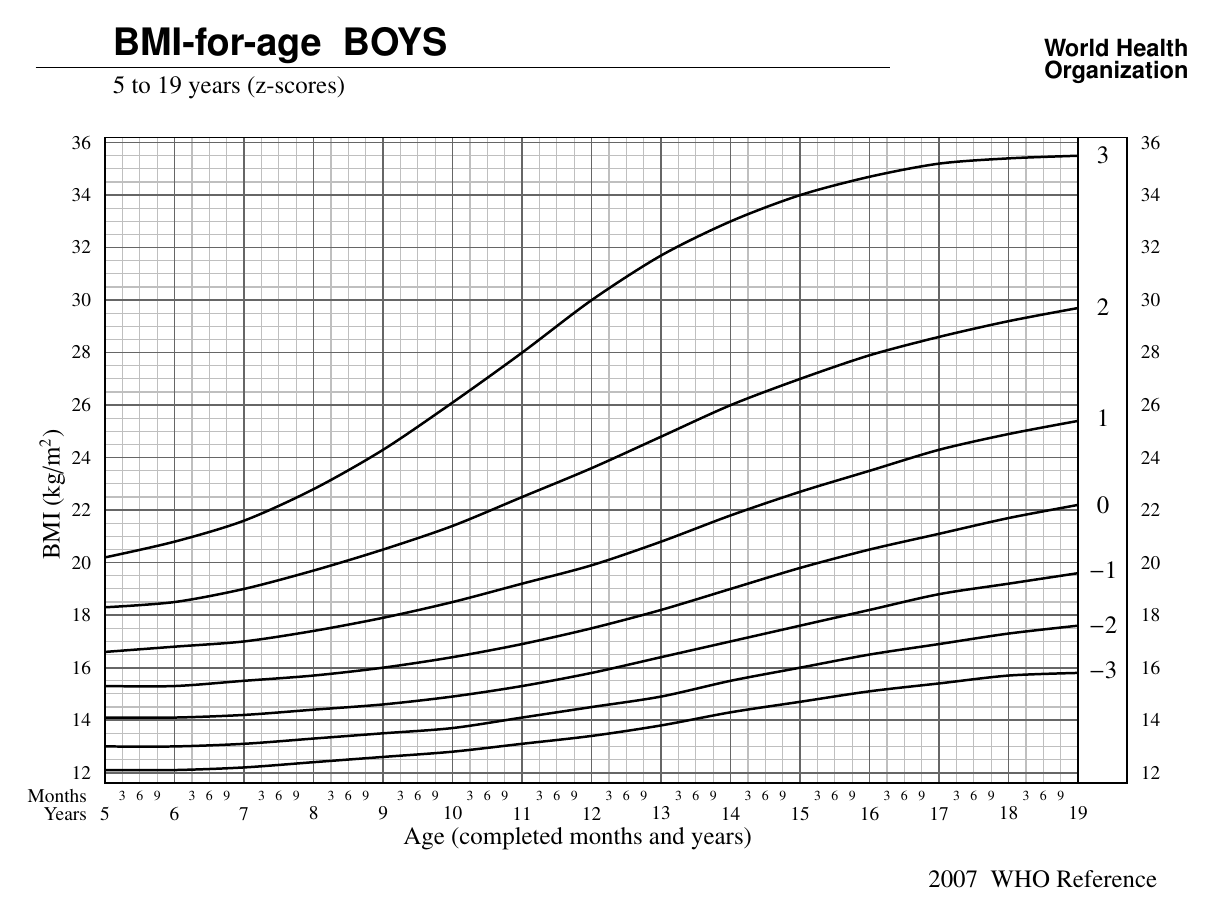
\begin{tikzpicture}[x=0.8827cm,y=0.3334cm]
\begin{scope}[shift={(-5,-12)}]
\foreach \a in {5,5.25,...,19}{\draw[black!25,line width=0.4pt] (\a,11.6) -- (\a,36.2);}
\foreach \b in {12,12.5,...,36}{\draw[black!25,line width=0.4pt] (5,\b) -- (19,\b);}
\foreach \a in {5,...,19}{\draw[black!60,line width=0.6pt] (\a,11.6) -- (\a,36.2);}
\foreach \b in {12,14,...,36}{\draw[black!60,line width=0.6pt] (5,\b) -- (19,\b);
  \node[font=\scriptsize,anchor=east,inner sep=1pt] at (4.85,\b) {\b};
  \node[font=\scriptsize,anchor=west,inner sep=1pt] at (19.85,\b) {\b};}
\draw (5,11.6) rectangle (19,36.2);
\draw (19,11.6) -- (19.7,11.6) -- (19.7,36.2) -- (19,36.2);
\foreach \a in {5,...,18}{\foreach \m in {3,6,9}{\node[font=\tiny,inner sep=0pt] at ({\a+\m/12},11.12) {\m};}}
\foreach \a in {5,...,19}{\node[font=\scriptsize,inner sep=0pt] at (\a,10.44) {\a};}
\node[font=\scriptsize,anchor=east,inner sep=0pt] at (4.75,11.12) {Months};
\node[font=\scriptsize,anchor=east,inner sep=0pt] at (4.75,10.44) {Years};
\node[font=\small] at (11.8,9.5) {Age (completed months and years)};
\node[font=\small,rotate=90] at (4.24,22.6) {BMI (kg/m$^2$)};
\foreach \c in {
 {(5,20.2)(6,20.8)(7,21.6)(8,22.8)(9,24.3)(10,26.1)(11,28.0)(12,30.0)(13,31.7)(14,33.0)(15,34.0)(16,34.7)(17,35.2)(18,35.4)(19,35.5)},
 {(5,18.3)(6,18.5)(7,19.0)(8,19.7)(9,20.5)(10,21.4)(11,22.5)(12,23.6)(13,24.8)(14,26.0)(15,27.0)(16,27.9)(17,28.6)(18,29.2)(19,29.7)},
 {(5,16.6)(6,16.8)(7,17.0)(8,17.4)(9,17.9)(10,18.5)(11,19.2)(12,19.9)(13,20.8)(14,21.8)(15,22.7)(16,23.5)(17,24.3)(18,24.9)(19,25.4)},
 {(5,15.3)(6,15.3)(7,15.5)(8,15.7)(9,16.0)(10,16.4)(11,16.9)(12,17.5)(13,18.2)(14,19.0)(15,19.8)(16,20.5)(17,21.1)(18,21.7)(19,22.2)},
 {(5,14.1)(6,14.1)(7,14.2)(8,14.4)(9,14.6)(10,14.9)(11,15.3)(12,15.8)(13,16.4)(14,17.0)(15,17.6)(16,18.2)(17,18.8)(18,19.2)(19,19.6)},
 {(5,13.0)(6,13.0)(7,13.1)(8,13.3)(9,13.5)(10,13.7)(11,14.1)(12,14.5)(13,14.9)(14,15.5)(15,16.0)(16,16.5)(17,16.9)(18,17.3)(19,17.6)},
 {(5,12.1)(6,12.1)(7,12.2)(8,12.4)(9,12.6)(10,12.8)(11,13.1)(12,13.4)(13,13.8)(14,14.3)(15,14.7)(16,15.1)(17,15.4)(18,15.7)(19,15.8)}}
 {\draw[line width=0.9pt] plot[smooth] coordinates \c;}
\foreach \z/\b in {3/35.5,2/29.75,1/25.5,0/22.2,-1/19.7,-2/17.6,-3/15.9}{\node[font=\small] at (19.36,\b) {$\z$};}
\node[font=\Large\bfseries\sffamily,anchor=west,inner sep=0pt] at (5.1,39.7) {BMI-for-age\ \ BOYS};
\draw (4,38.86) -- (16.3,38.86);
\node[font=\small,anchor=west,inner sep=0pt] at (5.1,38.1) {5 to 19 years (z-scores)};
\node[font=\small\bfseries\sffamily,anchor=east,align=right,inner sep=0pt] at (20.6,39.1) {World Health\\[-3pt]Organization};
\node[font=\small,anchor=east,inner sep=0pt] at (20.15,7.96) {2007\ \ WHO Reference};
\end{scope}
\end{tikzpicture}
\end{document}